
Przy implementacji języka TQL zastosowałyśmy podejście polegające na tzw. preprocessingu -- wzorzec Preprocessor \cite{mernik}.
W naszym przypadku polega to na przetłumaczeniu zapytania w języku TQL na zapytanie w innym, istniejącym już języku zapytań wyższego poziomu,
a następnie skorzystaniu z przetłumaczonego w ten sposób zapytania. W tej części pracy przedstawimy sposób zaimplementowania programu tłumaczącego.

Jednym z głównych założeń języka TQL, szczególnie ważnym z punktu widzenia implementacji, jest niezależność od struktury danych.
W związku z tym istotną cechą programu tłumaczącego zapytania w TQL (translatora) jest możliwość dostosowania  
go do współpracy z różnymi bazami danych.
%Jednym z głównych wymagań postawionych przed translatorem, żeby można było podłączyć różne bazy danych.
 Wynikiem tego jest podział translatora na 2 rodzaje modułów (rysunek \ref{moduly}):
\begin{enumerate}
 \item \textbf{Podstawowe} -- niezależne od struktury danych, zajmujące się głównie parsowaniem i analizą składniową zapytania.
 \item \textbf{Wymienne} -- zależne od struktury danych, tłumaczące zapytanie z TQL na język odpowiedni dla używanej bazy danych
i wywołujące je.
\end{enumerate}

\begin{figure}[h]
 \centering
 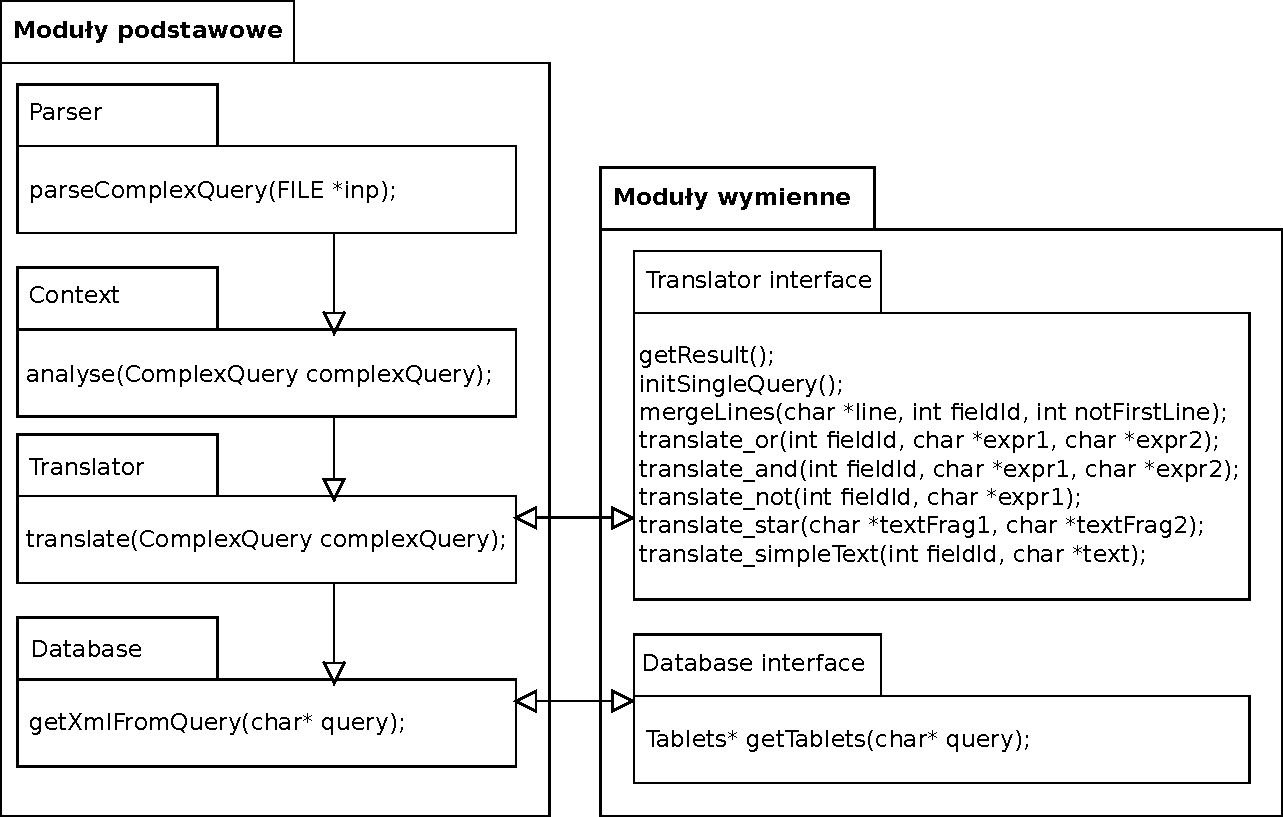
\includegraphics[width=450px]{../diagramy/pakiety.pdf}
 % pakiety.pdf: 585x300 pixel, 72dpi, 20.64x10.58 cm, bb=0 0 585 300
 \caption{Podział programu na moduły}
 \label{moduly}
\end{figure}


Na rysunku \ref{struktura_systemu} przedstawiamy ogólnie strukturę systemu, który korzysta z translatora TQL. Taki system, oprócz modułów podstawowych translatora, zawiera bazę tabliczek w dowolnej formie, implemetację modułów wymiennych umożliwiającą korzystanie z tej bazy, oraz interfejs użytkownika -- do wprowadzania zapytań i wyświetlania wyników. \\

 W niniejszej pracy prezentujemy dwie prototypowe implementacje translatora, zawierające własne zestawy modułów wymiennych: 
dla bazy PostgreSQL oraz XML.
Wybór modułów wymiennych odbywa się na poziomie kompilacji. Jest to rozwiązanie najprostsze do zaimplementowania,
jednak wymaga osobnego programu dla każdego rodzaju bazy danych.

 Stworzony przez nas Makefile domyślnie buduje obie implementacje translatora TQL.
%Bez względu na wybór modułu wymiennego interfejs całego translatora jest taki sam we wszystkich instancjach.

\begin{figure}[h]
 \centering
 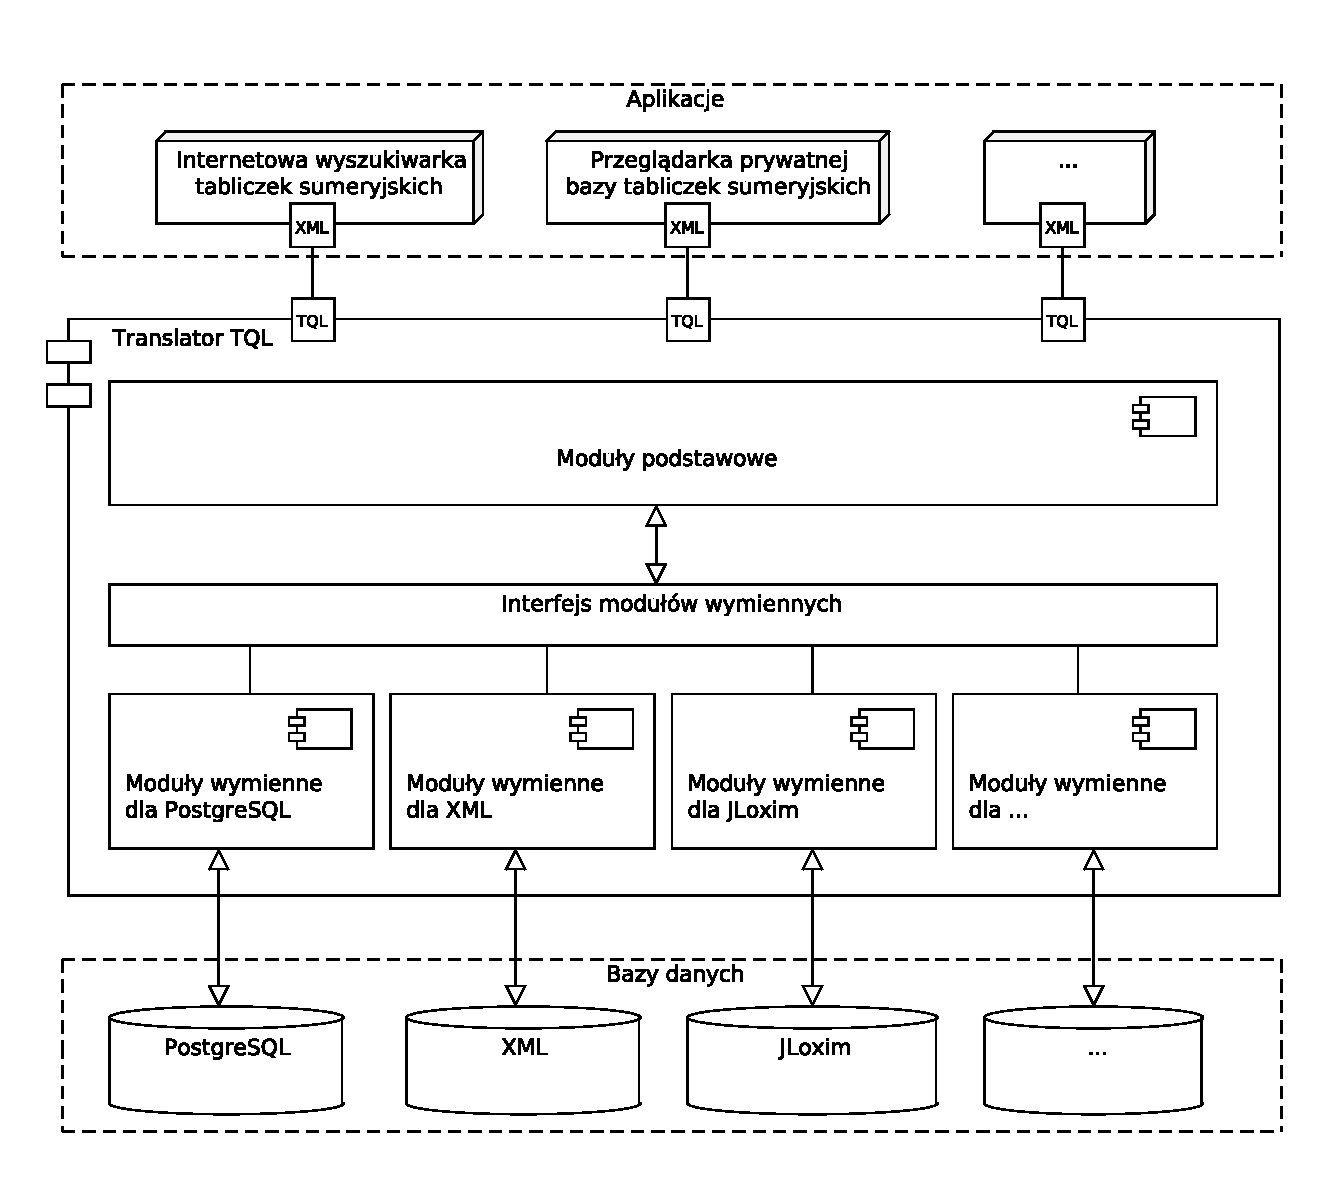
\includegraphics[width=450px,bb=0 0 608 517]{../diagramy/struktura2.pdf}
 % struktura.pdf: 608x517 pixel, 72dpi, 21.45x18.24 cm, bb=0 0 608 517
 \caption{Struktura systemu korzystającego z translatora}
 \label{struktura_systemu}
\end{figure}

\section{Moduły podstawowe}

W tym rozdziale przedstawimy dokładniej poszczególne moduły podstawowe translatora.

\subsection{Parser}
Parser został utworzony za pomocą narzędzia BNFC \cite{bnfc}. Na podstawie etykietowanej gramatyki BNF 
narzędzie to tworzy parser oraz szkielet analizatora składni w wybranym języku: C, C++, C\#, F\#, Haskell, Java lub OCaml. 
BNFC tworzy również pliki wejściowe dla generatora leksera (np. Flex) oraz dla generatora parsera (np. Bison). 
Dodatkowym produktem jest dokument w formacie Latex, który zawiera specyfikację zaprojektowanego języka.


Po automatycznym utworzeniu parsera, 
poprawiłyśmy nazwy stałych oznaczających symbole na bardziej intuicyjne.
Następnie
dodałyśmy tablicę symboli,
usunęłyśmy niepotrzebne funkcje z interfejsu
i ogólnie uporządkowałyśmy kod.

Moduł  parsuje zapytanie w języku TQL, tworząc drzewo struktury składniowej, które jest zdefiniowane w pliku pomocniczym Absyn.h.

Główna funkcja tego modułu to \verb|parseComplexQuery(FILE *inp)|. Argumentem jest wskaźnik do pliku zawierającego zapytanie TQL, 
a wynikiem odpowiednie drzewo struktury składniowej.

Na parser składają się następujące pliki:
\begin{itemize}
 \item Parser.cpp
 \item Parser.h
 \item TQL.y % tłumaczony na Parser.c
 \item TQL.l % tłumaczony na Lexer.c
\end{itemize}


\subsection{Analizator kontekstowy}
Podstawową funkcją w tym module jest \verb|analyse(ComplexQuery complexQuery)|, której argumentem oraz wynikiem jest 
drzewo struktury składniowej zapytania TQL. Funkcja ta
 sprawdza, czy podano prawidłowe nazwy pól, na podstawie których następuje wyszkukiwanie,  %to co jest po lewej w linii zapytania jest nazwą pola.
oraz upraszcza drzewo -- z wywołania zapytania (wywołanie \textit{search in}) tworzy zapytanie proste.

Analizator kontekstowy składa się z następujących plików:
\begin{itemize}
 \item Context.cpp
 \item Context.h
\end{itemize}

\subsection{Translator}
Zadaniem translatora jest przetłumaczenie drzewa składni abstrakcyjnej na zapytanie w docelowym języku.
Składa się z następujących plików:
\begin {itemize}
 \item Translator.cpp
 \item Translator.h
 \item Translator\_interface.h (interfejs modułu translatora zależnego od bazy danych)
 %\item Translator\_config.c (implementacja interfejsu z Translator\_config.h, zależny od wyboru bazy danych itp)
\end {itemize}

Tłumaczenie poszczególnych elementów drzewa zależy od implementacji interfejsu zawartego w pliku Translator\_interface.h. 
Funkcja \verb|translate(ComplexQuery complexQuery)| przechodzi całą strukturę drzewa, wywołując w razie 
potrzeby odpowiednie funkcje z Translator\_interface.
Następnie pobiera przetłumaczone zapytanie za pomocą funkcji getResult() i przekazuje je jako wynik.

\subsection{Baza}
Moduł bazy jest odpowiedzialny za wywołanie przetłumaczonego zapytania i przekazanie wyniku w określonej formie -- jako XML.
Składa się z następujących plików:
\begin {itemize}
 \item Database.cpp
 \item Database.h
 \item Database\_interface.h (interfejs modułu bazy zależnego od bazy danych)
% \item Database\_config.c (implementacja interfejsu z Database\_conf.h, zależny od wyboru bazy danych itp)
\end {itemize}

Główną funkcją w tym module jest \verb|getXmlFromQuery(char *query)|, która
wywołuje funkcję \verb|getTablets(char *query|) z Database\_interface.h, jako parametr podając przetłumaczoną treść zapytania. 
Dostaje w wyniku strukturę danych Tablets, wypełnioną informacjami o wyszukanych tabliczkach.
Następnie na podstawie otrzymanej struktury tworzy dokument XML i przekazuje go jako wynik wywołania zapytania.
\newline
Struktura Tablets zawiera metadane tabliczki, jej treść oraz informację o frazach, na podstawie których tabliczka została znaleziona. 
Poniżej przedstawiamy definicję struktury Tablets:
\begin{verbatim}
typedef struct{    
    char* id;
    char* id_cdli;
    char* publication;
    char* measurements;
    char* year;
    char* provenience;
    char* period;
    char* genre;
    char* subgenre;
    char* collection;
    char* text;
    Tags* tags; // specjalnie oznaczone miejsca w tekscie - frazy wyszukiwania
} Tablet;

typedef struct{
    int size;
    Tablet* tabs;
} Tablets;
\end{verbatim}

Zakładamy, że w bazie danych znajdują się informacje potrzebne do wypełnienia powyższej struktury (nie licząc fraz wyszukiwania).
%Wszystkie niezbędne informacje powinny się znajdować w bazie danych.

\subsection{Pliki pomocnicze}
Definicje struktur danych i funkcji służących do budowy drzewa struktury składniowej (wygenerowane za pomocą BNFC \cite{bnfc}, 
następnie uproszczone):
\begin{itemize}
 \item Absyn.cpp
 \item Absyn.h
\end{itemize}
Tablica symboli:
\begin{itemize}
 \item Symbols.cpp
\item Symbols.h
\end{itemize}
Obsługa błędów:
\begin{itemize}
 \item Err.cpp
\item Err.h
\end{itemize}
Moduł do dzielenia tekstu względem separatora, pobrany z internetu \cite{cexplode}:
\begin{itemize}
 \item Cexplode.cpp
 \item Cexplode.h
\end{itemize}


\section{Moduły wymienne}
Pliki zależne od wyboru konkretnej bazy danych to:
\begin{itemize}
 \item Translator\_$<$nazwa$>$.cpp -- dla modułu translatora
\item Database\_$<$nazwa$>$.cpp -- dla modułu bazy
\end{itemize}
Ich interfejsy są wspólne dla wszystkich baz danych.
